\section*{Response to Reviewer 1}


\subsection*{Major comments}

\subsubsection*{Comment 1}

\rc
This paper developed SatRain, the first AI-ready benchmark dataset for satellite-based detection and estimation of rain, snow, graupel, and hail. SatRain includes multi-sensor satellite observations representative of the major platforms currently used in precipitation remote sensing, paired with high-quality reference estimates from ground-based radars corrected using rain gauge measurements. The topic is very interesting and has important implications in prediction of urban weather.

The findings of this study are worth of publication in the SD after revision as following: There are various types of global precipitation, such as convective rain, frontal rain, orographic rain, and typhoon rain. When the author cited examples to verify the reliability of the dataset, the current results only included typhoon-related precipitation cases and their spatial distribution, which is insufficient. In fact, it is essential to fully assess whether this precipitation dataset can capture the temporal and spatial variation characteristics of these different precipitation types, thereby demonstrating the robustness of the dataset's results. Particular attention should be paid to whether the dataset can effectively characterize locally intense convective precipitation, which has a small spatial scale and strong suddenness.
\reply

\subsubsection*{Author response} \\

We agree with the reviewer that a precipitation benchmark dataset must
adequately represent both the spatial and temporal characteristics of
precipitation. However, it appears to be a misunderstanding that our current
evaluation is limited to typhoon-related events. The analyses shown in Figures
13 and 14 are based on 619 overpasses over the Austria domain, 2912 overpasses
over CONUS, and 600 overpasses over Korea. The CONUS and Korea test datasets
each span a full year, and the Austria dataset spans two years. As a result, the
testing data encompass a broad spectrum of precipitation conditions and capture
both spatial and temporal variability.

To further address the reviewer's concern and illustrate the retrievals'
performance across diverse precipitation regimes, we have added an additional
case study to the manuscript featuring a convective system over western CONUS.

\subsubsection*{Changes in Manuscript}

\begin{itemize}
  \item We have added the figure shown in Fig.~\ref{fig:case_study_1} and a paragraph discussing the results.
    \begin{change}[578]
        \DIFdelbegin \DIFdel{The retrieved precipitation fields are compared to the reference ground-based
        radar estimates and two baselines from the ERA-5 reanalysis dataset and }\DIFdelend \DIFaddbegin \DIFadd{Figure 11 presents the reference and retrieved surface
        precipitation fields for a quasi-linear convective system that developed on the
        afternoon of April 13, 2022 over the Southern and Midwestern United States. The
        reference field shows scattered pockets of intense convection in the southern
        portion of the domain, which merge into a quasi-linear system farther north. In
        contrast, weaker, scattered patches of stratiform precipitation occur in the
        northernmost part of the scene.
        }

        \DIFadd{Both the GPROF V7 baseline estimates and }\DIFaddend the \DIFdelbegin \DIFdel{GPROF precipitation retrieval in Fig.
        ~11. The results
        demonstrate that all retrievals capture the main precipitation structures }\DIFdelend \DIFaddbegin \DIFadd{SatRain-based retrievals capture
        the intense convective precipitation with high fidelity. Larger differences
        appear in the stratiform region to the north, particularly for the SatRain
        retrievals relying exclusively on visible and infrared observations. Despite
        this, all SatRain-based retrievals achieve strong accuracy metrics, with even
        the single-channel IR model surpassing the GPROF V7 baseline. ERA5 performs
        least well in representing the convective event: although it produces
        comparatively high rain rates in the south, these features are displaced
        relative to the reference, resulting in an elevated mean-squared error and a low
        linear correlation coefficient.
        }

    \end{change}
   \item We have also rephrased the introductory paragraph of Section~4.2 to highlight the size and temporal extent of the  test set.
     \begin{change}[616]
        The \DIFaddbegin \DIFadd{ML }\DIFaddend models trained on the CONUS dataset were further evaluated \DIFdelbegin \DIFdel{against three independent test domains }\DIFdelend \DIFaddbegin \DIFadd{using all test
        scenes from the three test regions }\DIFaddend (CONUS, Austria, and Korea). The \DIFdelbegin \DIFdel{results, displayed }\DIFdelend \DIFaddbegin \DIFadd{test set
        includes 619 overpasses over the Austria domain, 600 over the Korea domain, and 2912
        over the CONUS domain, covering one year for CONUS and Korea and two years for
        Austria. As shown }\DIFaddend in Fig.~12, \DIFdelbegin \DIFdel{are consistent }\DIFdelend \DIFaddbegin \DIFadd{the results align }\DIFaddend with
        the case \DIFdelbegin \DIFdel{study presented
        }\DIFdelend \DIFaddbegin \DIFadd{studies discussed }\DIFaddend above. The SatRain-based GMI retrieval consistently
        outperforms the GPROF V7 baseline, \DIFdelbegin \DIFdel{despite relying }\DIFdelend \DIFaddbegin \DIFadd{even though both rely }\DIFaddend on the same \DIFaddbegin \DIFadd{input
        }\DIFaddend observations. Retrievals \DIFdelbegin \DIFdel{based on
        }\DIFdelend \DIFaddbegin \DIFadd{using }\DIFaddend geostationary measurements (\DIFdelbegin \DIFdel{GEO and GEO-IR)
        achieve lower accuracy overall but
        still surpass }\DIFdelend \DIFaddbegin \DIFadd{Geo and Geo-IR)
        exhibit lower overall accuracy but still perform better than }\DIFaddend the ERA5 baseline.
        \DIFdelbegin \DIFdel{These improvements across multiple domains
        confirm both the technical soundness and the practical value of SatRain.
        }\DIFdelend
    \end{change}

\end{itemize}

\begin{figure}[htbp] % h=here, t=top, b=bottom, p=page of floats
	\centering
	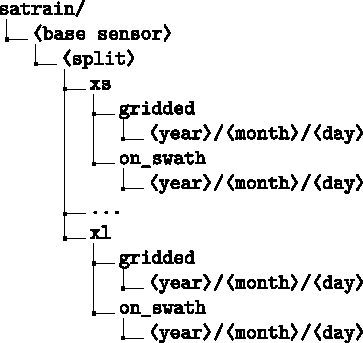
\includegraphics[width=1.0\textwidth]{figures_revised/fig09.pdf}
	\caption{ Precipitation retrievals for a quasi-linear convective system,
	  comparing models trained on the SatRain dataset with ground-based
	  precipitation estimates and two baseline products. Panel (a) shows the
	  ground-based reference precipitation, panel (b) the ERA5 reanalysis, and
	  panel (c) the GPROF V7 retrieval applied to GMI observations. Panels (d),
	  (e), and (f) present SatRain-trained retrievals using single-channel IR
	  observations (Geo-IR), multi-channel Vis and IR observations (Geo), and
	  GMI PMW observations, respectively. }
	\label{fig:case_study_1}
\end{figure}
